\chapter{Basicness}
\section{How Shall a Thing be Called?}

Nel nostro mondo esistono parole semplici, facili da imparare e da ricordare, che si riferiscono a concetti comuni. Nel 1958, Roger Brown scrisse un articolo: "How Shall a Thing be Called?" in cui si pose la domanda "Come si scelgono dei termini per definire oggetti e concetti?". Molti concetti sono complessi e quindi è difficile trovare dei termini adatti per descriverli. Al giorno d'oggi non si ha ancora una risposta a questa domanda. Nel 1930, Ogden studio approfonditamente il concetto di \fancyglitter{Basic level}, il \textit{vocabolario di base}. Egli propose un insieme di parole costituenti la base della comunicazione. Negli stessi anni Brown cercava di capire i criteri secondo cui una parola fosse basica o meno (fig: \ref{fig:bas}):

\begin{itemize}
  \item Parole corte. 
  \item Concetti concreti. 
  \item Facili da pronunciare. 
  \item Frequentemente usate. 
\end{itemize}
\begin{figure}[h]
    \centering
    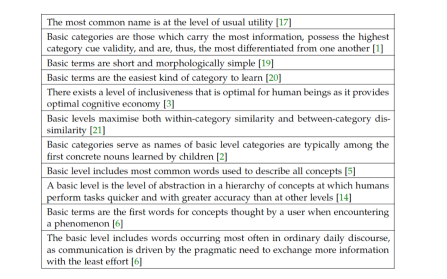
\includegraphics[scale=0.65]{05/basic.png}
    \caption{Alcune definizioni di Basicness.}
    \label{fig:bas}
\end{figure}

\paragraph{Considerazioni:}

\begin{itemize}
  \item Sopravvivenza sociale: l'acquisizione del vocabolario di base è essenziale per i \textit{second language learner} per poter comunicare i propri bisogni. 
  \item Legame termine-concetto: purtroppo non tutti i concetti sono facilmente descritti da un termine. Inoltre alcuni termini basic possono essere usati per concetti avanzati. Per esempio cane che ha un significato in termini militari. 
  \item Soggettività: il livello base è estremamente soggettivo poiché gli stessi termini sono interpretati in maniera diversa da persone diverse. 
  \item Advanced: i termini advanced vengono definiti in materia di basic. Tutto ciò che non è basic è advanced. 
\end{itemize}








